\subsection{Der Lehrer und Schulleiter}

1929 wurde August Högn zum
Oberlehrer ernannt. Dieser höhere Dienstgrad hatte ebenso wie seine
Ernennung zum Rektor 1940 bezüglich seines Aufgabenfeldes in der Schule
keinen Einfluss, da er schon seit 1921 Schulleiter war. Es war sicher
zur damaligen Zeit keine leichte Aufgabe, die Landschule zu leiten. Zum
einem war die finanzielle Lage der beteiligen Gemeinden, der so
genannten Schulsprengelverwaltung ziemlich angespannt, die für die
Instandsetzung der Schulgebäude einschließlich der Lehrerwohnungen und
die Beschaffung von Lehrmittel zuständig war. \footnote{Dokument Nr.
146, Brief von August Högn an Bürgermeister Forster, Ruhmannsfelden,
18.5.1936}

Zu manchen Zeiten wurden nicht einmal die notwendigen Lehrmittel im
erforderlichen Maße bereitgestellt. \footnote{Dokument Nr. 146, Brief
von August Högn an Bürgermeister Forster, Ruhmannsfelden, 18.5.1936}
Die finanziellen Engpässe wirkten sich natürlich ebenso auf den Zustand
der Schulgebäude aus. So konnten beispielsweise im Jahr 1934 die
Toiletten im so genannten Mädchenschulhaus eine Zeit lang gar nicht
mehr benutzt werden, da sie derart baufällig waren, dass laut Högn ihre
Benutzung lebensgefährlich für die Kinder war. \footnote{Dokument Nr.
144, Brief von August Högn an verstärkten Gemeinderat Ruhmannsfelden,
13.9.1934} Zum anderem schlug sich die schwierige Erwerbslage vieler
Familien negativ auf das Lernklima nieder. Besonders zur Erntezeit
mussten viele Kinder in der Landwirtschaft ihrer Eltern mithelfen, da
sich kaum eine Familie eine zusätzliche Arbeitskraft leisten konnte.
Aus diesem Grund war es zeitweise üblich, dass in den Sommermonaten der
Unterricht gekürzt werden musste. \footnote{Interview Nr. 6, Wilhelm
Ederer, 2.1.2003, Absatz 30} Eine dauerhafte Belastung für den
Schulbetrieb waren die langen Schulwege, die die Schüler aus am Rande
des großen Schulsprengels gelegenen Ortschaften und Höfen zu Fuß
zurücklegen mussten. Über eine Stunde dauernde Märsche zur Schule waren
keine Seltenheit und wurden bei Regen oder Schnee für die Schüler zur
Tortur. \footnote{Interview Nr. 6, Wilhelm Ederer, 2.1.2003, Absatz 10}

\begin{center}
\begin{minipage}{10.931cm}
\begin{flushleft}
\tablefirsthead{}
\tablehead{}
\tabletail{}
\tablelasttail{}
\begin{supertabular}{m{10.731cm}}

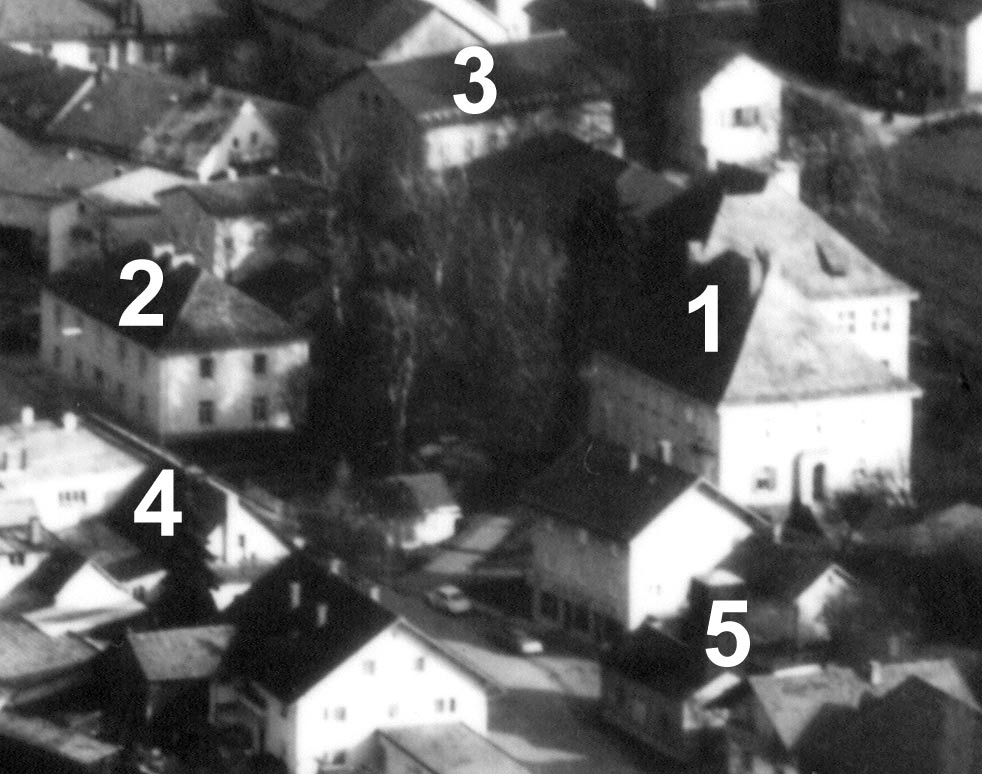
\includegraphics[width=10.548cm,height=8.313cm]{pictures/zulassungsarbeit-img030.jpg}

Schul- und Wohnhäuser von Högn:
\textbf{1:} Schulhaus von 1908: Hier wohnte August Högn 1932 – 1945,
\textbf{2:} Knabenschulhaus von 1834: Wohnung 1910 – 1932, \textbf{3:}
Mädchenschulhaus von 1884, \textbf{4:} Härtl-Haus: Wohnung 1945 – 1961,
\textbf{5:} Feuerwehrhaus\\
\end{supertabular}
\end{flushleft}
\end{minipage}
\end{center}

\begin{figure}
\img{}
\caption{}
\end{figure}

Wahrscheinlich lag es an den damals geringeren Anforderungen, die man an
eine Landschule stellte – überspitzt formuliert, war man schon froh,
wenn die Schüler regelmäßig am Unterricht teilnahmen – und an der
Positionen Högns als Schulleiter, dass er sich gewisse Dinge erlauben
konnte, die nicht regelkonform waren und in der heutigen Zeit undenkbar
wären. So ließ er beispielsweise die Schüler nicht nur für schulische
Zwecke, sondern auch für seine Privatangelegenheiten kleine Dienste und
Arbeiten während der Unterrichtszeit erledigen. Zu diesen Arbeiten
gehörten unter anderem einen Zettel von Klassenzimmer zu Klassenzimmer
tragen, \footnote{Interview Nr. 4, Maria Schröck, 30.12.2002, Absatz
46} Lehrmittel aus dem entsprechenden Zimmer holen, \footnote{Interview
Nr. 14, Johann Freisinger, 29.12.2003, Absatz 26} den Schulhof
aufräumen, das Pflaster am der Schule nahe gelegenen Kriegerdenkmal
ausgrasen \footnote{Interview Nr. 4, Maria Schröck, 30.12.2002, Absatz
14} und Holzaufrichten. \footnote{Korrespondenz Nr. 26, Brief von Franz
Danziger an Josef Friedrich, 25.2.2003; Interview Nr. 17, Max Holler,
26.8.2004, Absatz 16} Dies waren Dienste, die mit der Schule einen
gewissen Zusammenhang hatten, aber die Teppiche aus Högns Wohnung
klopfen, \footnote{Interview Nr. 6, Wilhelm Ederer, 2.1.2003, Absatz
34} von Högn geschossenes Wildfleisch zum Bahnhof bringen,\footnote{
Interview Nr. 17, Max Holler, 26.8.2004, Absatz 8} sein Rad
putzen \footnote{Interview Nr. 14, Johann Freisinger, 29.12.2003,
Absatz 24} oder sogar es reparieren \footnote{Interview Nr. 17, Max
Holler, 26.8.2004, Absatz 8} waren Arbeiten, die rein ins Private
fielen und jeden Bezug zur Schule entbehrten. Diese Tätigkeiten wurden
aber nicht als Strafarbeit, sondern als Zeichen besonderen Vertrauens
verstanden. \footnote{Korrespondenz Nr. 26, Brief von Franz Danziger an
Josef Friedrich, 25.2.2003}

{\centering
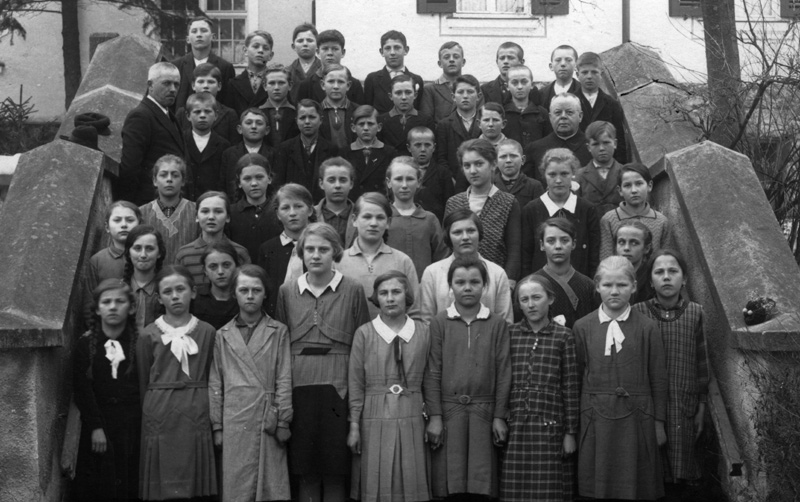
\includegraphics[width=16.044cm,height=10.081cm]{pictures/zulassungsarbeit-img031.jpg}
 \par}
Klassenfoto von 1932 mit August Högn
(links) und Pfarrer Fahrmeier (rechts)

Seitdem 1920 der Kirchendienst der Lehrer abgeschafft wurde, war der
Einsatz Högns als Organist bei Beerdigungen während der Unterrichtszeit
ein eindeutiger Verstoß gegen das damalige Schulrecht. Dass diese
Praxis auch noch zur NS-Zeit von den Behörden und der Seite der Eltern
toleriert wurde, lag an der besonders großen Macht der Institution
Kirche am Land. Eine gewöhnliche Beerdigung dauerte von 9 bis 11 Uhr,
so genannte „levitierte“ Beerdigungen für wohlhabende Verstorben
dauerten wesentlich länger. \footnote{Interview Nr. 4, Maria Schröck,
30.12.2002, Absatz 10} Högns Schüler mussten während seiner Abwesenheit
in Stillarbeit Aufgaben erledigen, ein paar Schüler wurden zu
Aufpassern ernannt \footnote{Interview Nr. 6, Wilhelm Ederer, 2.1.2003,
Absatz 8, Interview Nr. 4, Maria Schröck, 30.12.2002, Absatz 12;} und
die Lehrer der benachbarten Klassen statteten der „verwaisten Klasse“
hin und wieder einen Besuch ab. \footnote{Interview Nr. 4, Maria
Schröck, 30.12.2002, Absatz 10} Natürlich verhielten sich die Schüler
nicht nach Högns Vorstellung. Tumult im Klassenzimmer war noch das
kleinere Übel. Manchmal kam es sogar vor, dass sich einige Schüler
bereits auf den Nachhauseweg gemacht hatten, ehe Högn von der Kirche
ins Klassenzimmer zurückkehrte. Högn soll bei derartigen Vorkommnissen
des Öfteren versucht haben, diese Schüler mit dem Fahrrad einzuholen
und sie so zur Schule zurückzubringen. \footnote{Interview Nr. 6,
Wilhelm Ederer, 2.1.2003, Absatz 8}

\begin{center}
\begin{minipage}{6.202cm}
\begin{center}
\tablefirsthead{}
\tablehead{}
\tabletail{}
\tablelasttail{}
\begin{supertabular}{m{6.0020003cm}}

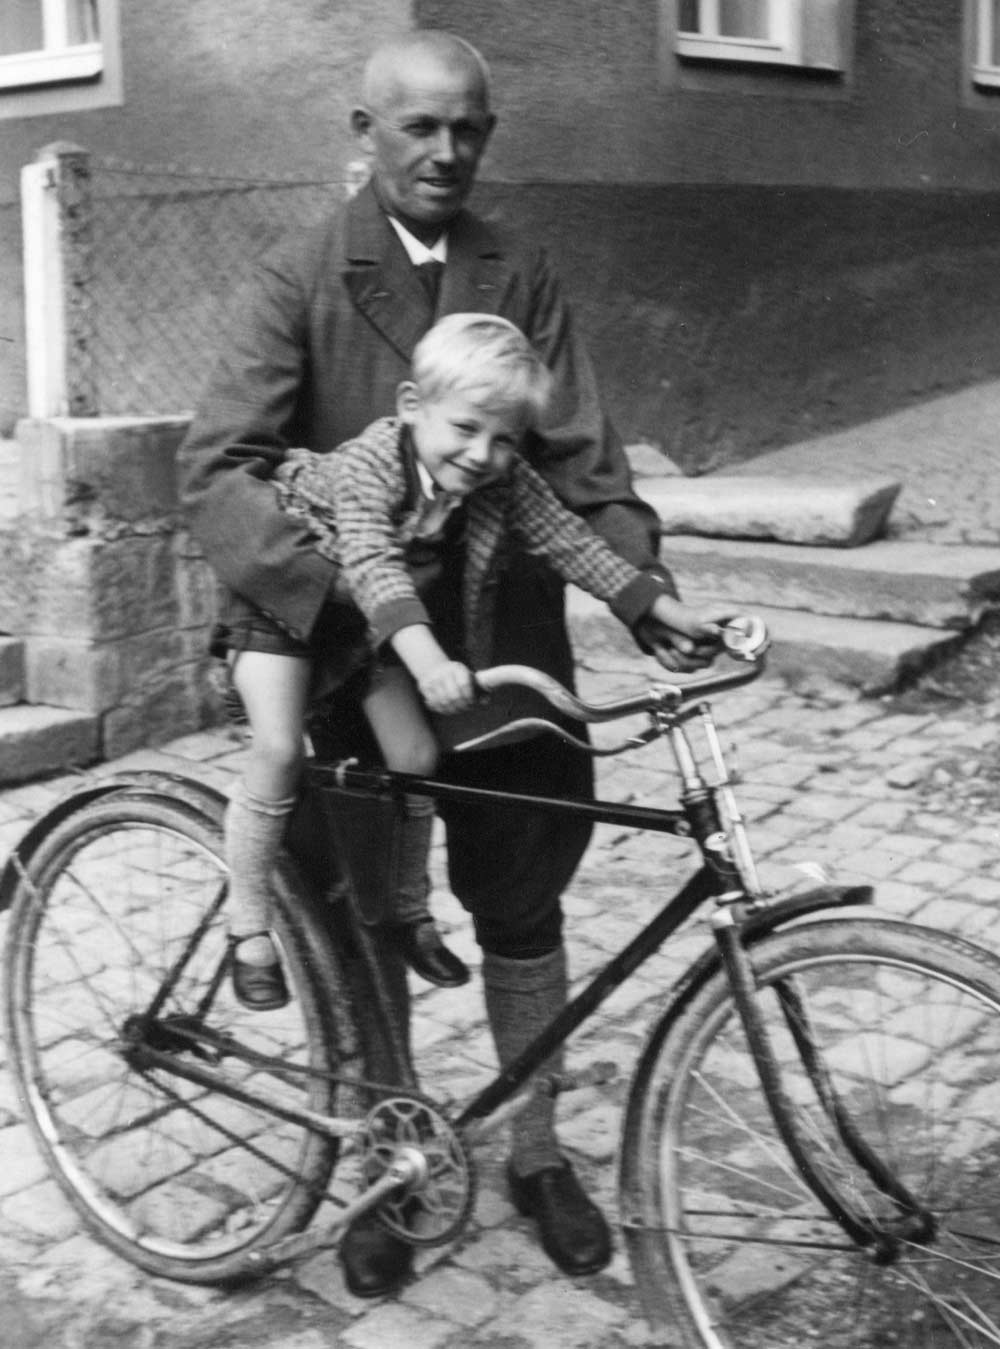
\includegraphics[width=5.821cm,height=7.851cm]{pictures/zulassungsarbeit-img032.jpg}

August Högn mit Enkel Werner
Schlumprecht und seinem Fahrrad 1939\\
\end{supertabular}
\end{center}
\end{minipage}
\end{center}
Die alltäglichen Beschwerlichkeiten, mit denen der damalige Lehrerstand
über all in Bayern zu kämpfen hatte – man bedenke die große
Schüleranzahl in einer Klasse – und die besonderen Schwierigkeiten in
Ruhmannsfelden schienen sich unter anderem auch in der Art
niedergeschlagen zu haben, wie Högn in der Klasse für Disziplin sorgte.
Viele der befragten Zeitzeugen bezeichneten August Högn als strengen
Lehrer. \footnote{Interview Nr. 3, Ida Högn,
29.12.2002, Absatz 6; Interview Nr. 14, Johann Freisinger, 29.12.2003,
Absatz 2; Interview Nr. 17, Max Holler, 26.8.2004, Absatz 16; Interview
Nr. 5, Barbara Essigmann, 2.1.2003, Absatz 18; Interview Nr. 24, Johann
Glasschröder, 28.12.2004, Absatz 12, 28} Dass er unfolgsame Schüler
mit Ohrfeigen, Tatzen \footnote{Interview Nr. 17, Max Holler,
26.8.2004, Absatz 12}, Ziehen an den Haarspitzen \footnote{Interview
Nr. 5, Barbara Essigmann, 2.1.2003, Absatz 20} und Schlägen auf den
Hintern \footnote{Interview Nr. 5, Barbara Essigmann, 2.1.2003, Absatz
18} bestrafte, ist daher kaum verwunderlich und außerdem üblich für die
damalige Zeit. Noch gewalttätigere Maßnahmen sind von ehemaligen
Schülern als Zeichen einer gewissen Hilflosigkeit verstanden worden,
die sie beim alternden und überforderten Lehrer beobachten konnten.
Hierzu gehörten Strafen, wie zum Beispiel Schülern die Schiefertafel so
stark über den zu Kopf schlagen, dass sie zerbrach, \footnote{Interview
Nr. 3, Ida Högn, 29.12.2002, Absatz 6} einen Bund mit vielen Schlüsseln
über den Kopf schlagen, \footnote{Interview Nr. 14, Johann Freisinger,
29.12.2003, Absatz 6} den Kopf der Schüler an die Tafel
stoßen, \footnote{Interview Nr. 14, Johann Freisinger, 29.12.2003,
Absatz 26; Interview Nr. 6, Wilhelm Ederer, 2.1.2003, Absatz 16} oder
sogar mit einem Blumentopf nach einem Schüler werfen.\footnote{
Interview Nr. 14, Johann Freisinger, 29.12.2003, Absatz 28} Ebenso gut
passen ungewöhnlich scharfe Beschimpfungen der Schüler mit Ausdrücken
wie etwa „ordinärer Hund“, \footnote{Interview Nr. 6, Wilhelm Ederer,
2.1.2003, Absatz 16} „dreckiger Hundschuft“ \footnote{Interview Nr. 17,
Max Holler, 26.8.2004, Absatz 16} oder „blöder Hammel“ \footnote{
Interview Nr. 5, Barbara Essigmann, 2.1.2003, Absatz 20} zum Bild des
alternden und überforderten Lehrers. Doch nicht nur mit harten Strafen,
die sich fester ins Gedächtnis ehemaliger Schüler eingruben, als
mancher pädagogische Kniff, versuchte er für Ruhe im Klassenzimmer zu
sorgen. Als geschickter Lehrer zeigte er sich, wenn er die Schüler am
Ende jeder Unterrichtsstunde zur Entspannung und Auflockerung aufstehen
ließ, um ihre überschüssigen Energien vor und nicht während der Stunde
loszuwerden. \footnote{Korrespondenz Nr. 26, Brief von Franz Danziger
an Josef Friedrich, 25.2.2003} Das negative Bild vom strafenden Lehrer
hebt sich auf, wenn Zeitzeugen ihren ehemaligen Lehrer trotz aller
seiner Wutausbrüche als sehr gerechten Lehrer bezeichnen.\footnote{
Interview Nr. 24, Johann Glasschröder, 28.12.2004, Absatz 12}

Als Entschädigung für manche Schwierigkeit im Schulalltag galt für den
leidenschaftlichen Musiker sicher der Musikunterricht. Dieser hatte den
größten Stellenwert unter allen Fächern, die Högn
unterrichtete. \footnote{Interview Nr. 17, Max Holler, 26.8.2004,
Absatz 10; Interview Nr. 4, Maria Schröck, 30.12.2002, Absatz 10;
Korrespondenz Nr. 26, Brief von Franz Danziger an Josef Friedrich,
25.2.2003} Zu manchen Zeiten wurde jeden Tag eine Stunde
gesungen. \footnote{Interview Nr. 5, Barbara Essigmann, 2.1.2003,
Absatz 20} Selbst als kurz vor Ende des 2. Weltkriegs ein Lehrer zwei
Klassen unterrichten musste – eine Klasse hatte täglich nur drei
Stunden Unterricht – wurde jeden Tag vor Beginn des Unterrichts statt
des Gebets ein Lied gesungen. \footnote{Interview Nr. 16, Maria
Freisinger, 25.8.2004, Absatz 22} Da die Volksschule Ruhmannsfelden
kein Klavier besaß, begleitete Högn die Volkslieder normalerweise auf
der Violine. \footnote{Interview Nr. 4, Maria Schröck, 30.12.2002,
Absatz 8; Interview Nr. 5, Barbara Essigmann, 2.1.2003, Absatz 20} Es
kam aber auch vor, dass die Lieder unbegleitet gesungen
wurden. \footnote{Interview Nr. 16, Maria Freisinger, 25.8.2004, Absatz
26} Nach Aussagen mehrerer ehemaliger Schüler sang man unter August
Högn durchaus mehrstimmig. \footnote{Interview Nr. 5, Barbara
Essigmann, 2.1.2003, Absatz 42; Interview Nr. 17, Max Holler,
26.8.2004, Absatz 42} Ein anfangs dreistimmiges, zum Schluss hin sogar
teilweise fünfstimmiges Arrangement Högns von dem Lied „Tauet Himmel“,
das mit „aus meinen Kinderliedern“ überschrieben ist, bestätigt dies.
Eine ehemalige Schülerin kann sich sogar an den Fall erinnern, als Högn
speziell für ihre Banknachbarin eine zweite Stimme arrangierte: Die
Schülerin sang einmal spontan zu einem einstimmigen Volkslied eine
zweite Stimme. Schon am nächsten Schultag legte ihr Högn eine
ausgeschriebene zweite Stimme vor. \footnote{Interview Nr. 16, Maria
Freisinger, 25.8.2004, Absatz 24} Beim Singen legte August Högn
durchaus Wert auf Stimmbildung. Er verlangte zum Beispiel, dass mit
Bruststimme \footnote{Interview Nr. 4, Maria Schröck, 30.12.2002,
Absatz 8} und im Stehen gesungen wurde, da sich so die
\zitat{„Lungen besser weite“} \footnote{Interview Nr. 5, Barbara Essigmann, 2.1.2003, Absatz
42}\zitat{ }könnten. Den Schülern standen Liederbücher zur
Verfügung, aus denen sie sich durchaus selbst Lieder zum Singen
aussuchen durften. \footnote{Interview Nr. 16, Maria Freisinger,
25.8.2004, Absatz 22} Es handelte sich wahrscheinlich um ein damals
gängiges Repertoire an allgemein bekannten Volksliedern, das gemeinsam
musiziert wurde. \footnote{Interview Nr. 5, Barbara Essigmann,
2.1.2003, Absatz 20} Aber auch politische Lieder wurden gesungen. Eine
Zeitzeugin berichtete, dass um 1930, also zur Zeit der
Rheinlandbefreiung und dem Aufkommen der deutsch-nationalen Bewegung,
häufiger patriotische Lieder wie z. B. das Lied „Kräftiger Zweig der
deutschen Eiche“ gesungen wurden. \footnote{Interview Nr. 4, Maria
Schröck, 30.12.2002, Absatz 6} Ab 28.12.1938 war der „Singkamerad“
 \footnote{Seite 129} das einzige an den bayerischen Volksschulen
zugelassene Liederbuch und von diesem Zeitpunkt an konnte man Lieder
vor allem mit NS-Gedankengut aus den Klassenzimmern hören. Högns
Klassen bildeten hier keine Ausnahme. \footnote{Interview Nr. 17, Max
Holler, 26.8.2004, Absatz 12}

\begin{center}
\begin{minipage}{8.807cm}
\begin{flushleft}
\tablefirsthead{}
\tablehead{}
\tabletail{}
\tablelasttail{}
\begin{supertabular}{m{8.607cm}}

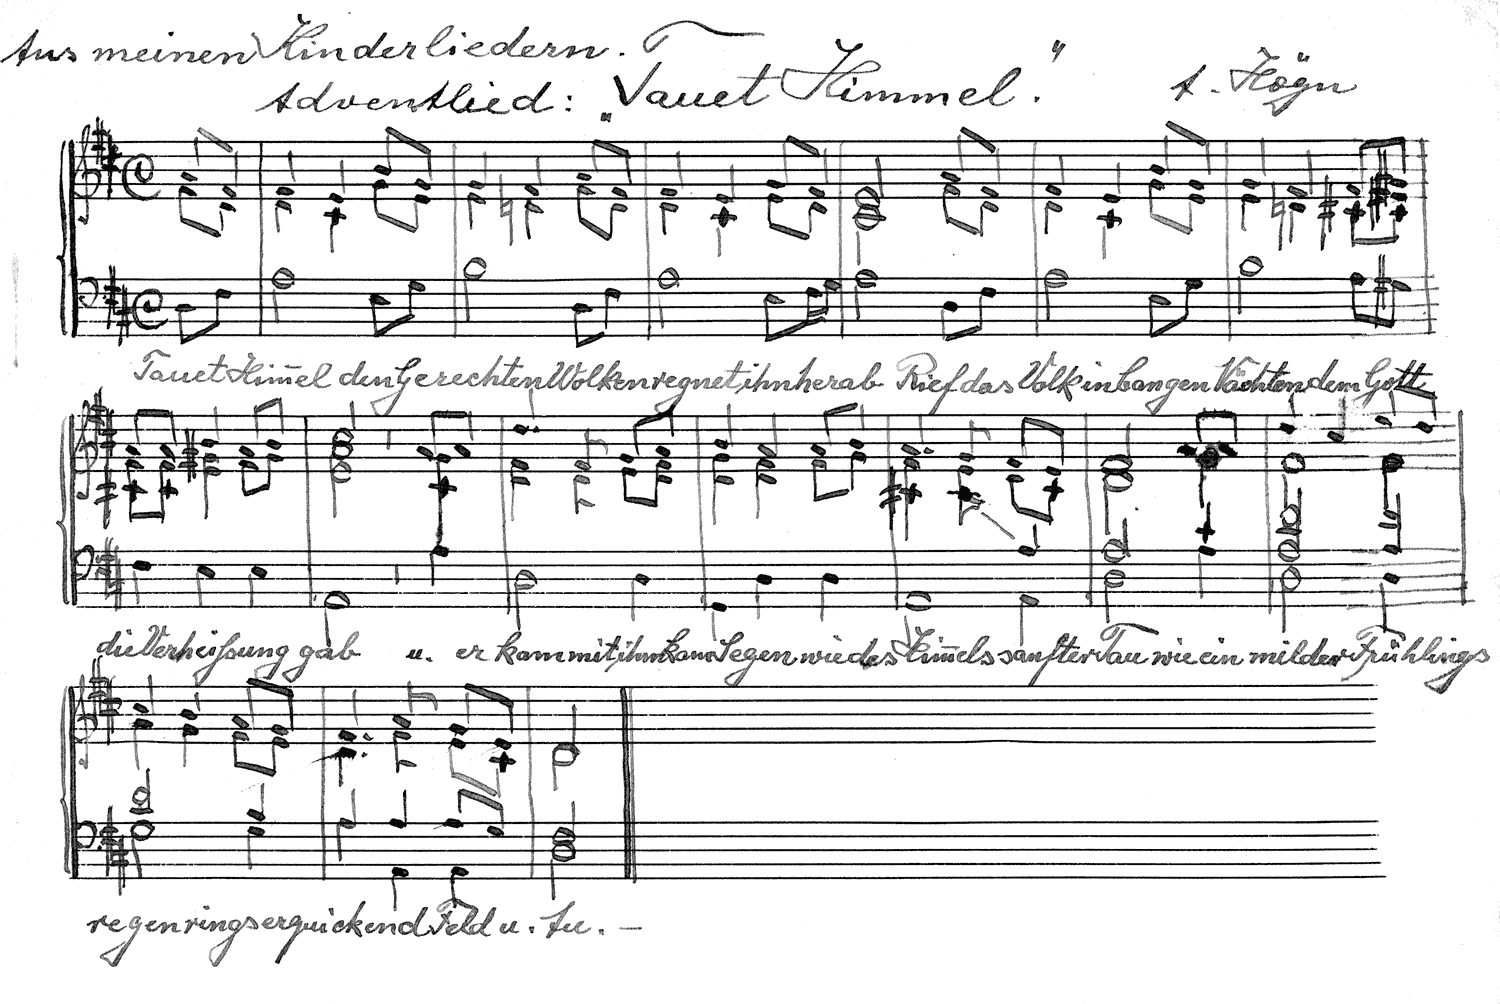
\includegraphics[width=8.373cm,height=5.604cm]{pictures/zulassungsarbeit-img033.png}

Arrangement des Liedes „Tauet Himmel“
von August Högn für den Schuleinsatz\\
\end{supertabular}
\end{flushleft}
\end{minipage}
\end{center}
